%% -*-latex-*-
\makeatletter
\declare@file@substitution{revtex4-1.cls}{revtex4-2.cls}
\makeatother
\documentclass{aastex631}
\let\tablenum\relax
\usepackage[separate-uncertainty=true]{siunitx}
\usepackage[utf8]{inputenc}
\begin{document}

\author{Andrew Ivanov}
\affiliation{Department of Astronomy, University of Washington, Seattle, WA 98195, USA}
\author{Nian Tong}
\affiliation{Department of Astronomy, University of Washington, Seattle, WA 98195, USA}
\date{\today}
\title{Pulsations of the ZZ Ceti star J1903+6035}

\begin{abstract}
We confirm the newly discovered pulsations of the J1903+6035 white
dwarf using the 0.5-m Astrophysical Research Consortium Small Aperture
Telescope (ARCSAT).  In 2020, Vincent et al., using a 2.6-m telescope,
acquired high-speed photometric observation of J1903+6035; from the
light curve with complex features, they deduced the presence of a
dominant \SI{726}{\second} pulsation mode. While the use of a
relatively large telescope allowing for fast (\SI{10}{\second} or
shorter) exposures makes producing a light curve with good
signal-to-noise ratio relatively easy, reliably detecting pulsations
of high-amplitude ZZ Ceti stars having dominant mode periods greater
than \SI{250}{\second} through small-diameter telescopes requiring
significantly longer exposures (exceeding \SI{100}{\second}) is also
possible. We demonstrate such observation using J1903+6035 as an
example, outline a possible data reduction approach and discuss its
applicability and shortcomings when observing similar objects. We
estimate the average period of the dominant mode of J1903+6035 at
$\SI{765\pm 29}{\second}$, which is within 5\% of the value reported
in the previous study. Finally, we provide a brief survey of the
current theoretical models describing ZZ Ceti pulsators and discuss
several important indirect observations that become possible through
precise measurements of their pulsation modes.
\end{abstract}
\section{Introduction}
\emph{ZZ Ceti}(also known as DAV) stars are hydrogen-rich white dwarfs
(WD) that exhibit non-radial pulsations. Typical periods of these
pulsations range between \(\SI{100}{\second}\) and
\(\SI{2000}{\second}\), and are always a combination of several
\emph{g}-mode (gravity wave) oscillations. For instance the
oscillations, of the first confirmed ZZ Ceti, HL Tau 76, are dominated
by two modes with periods \SI{746.2}{\second} and \SI{494.2}{\second}
\citep{Koester_1990}. More data on a number of early discovered
\emph{ZZ Ceti}, along with accessible theoretical explanations of the
nature of their variability (some of which may be obsolete as of
today) is given in \citet{Bradley_1998}.

All WDs are expected to pass the \emph{ZZ Ceti} instability strip at
some point during their lifetime and it is estimated that 98\% of all
stars end their lives as white dwarfs \citep{Catelan_2015}. It is also
believed that most or all stars of the DA spectral type pass the
\emph{ZZ Ceti} instability strip where they inevitably (\emph{ZZ Ceti}
being a \emph{pure} instability strip) develop \emph{g}-mode
oscillations while continuing to cool down. Thus, the pulsations of ZZ
Ceti stars provide an excellent window into the properties and
evolution of WD stars in general as well as offer means for making
other important indirect observations based on the cooling timescales
of degenerate stars. The the exact shape of the \emph{ZZ Ceti}
instability strip, from both theoretical and empirical standpoints, is
still an open question. On the observational side, this is in part
complicated by the lack of agreement with respect to various
assumptions made by researchers and also by substantial reduction in
the pulsation amplitude in stars near the edges of the strip, which
makes observation difficult or impossible. On the theoretical front,
the main challenge is the scarcity of high-resolution data necessary
for validating theoretical models.

The multi-mode nature of ZZ Ceti star pulsations along with the
observed negative correlation between the dominant period and the
amplitude of variation \citep{Vincent_2020} makes producing light
curves with reasonable time resolution difficult even for relatively
slow pulsators. Our best achievable time resolution of about
\(\SI{118}{\second}\) certainly wouldn't allow resolving all the modes
of J1903+6035; however, we demonstrate the possibility of detecting
the average period of the most prominent modes by means of
differential photometry followed by simple Fourier analysis or the
applications of the more advanced Lomb-Scargle periodogram algorithm
\citep{VanderPlas_2018}. We show that our analysis produces a result
consistent with that from \citet{Vincent_2020} shown in Figure
\ref{fig:vincent}, and discuss further steps and improvements to the
observation and data reduction techniques which could be helpful to
amateur astronomers interested in identifying new candidate DAV white
dwarfs through small telescopes.
\begin{figure}[htbp]
\centering
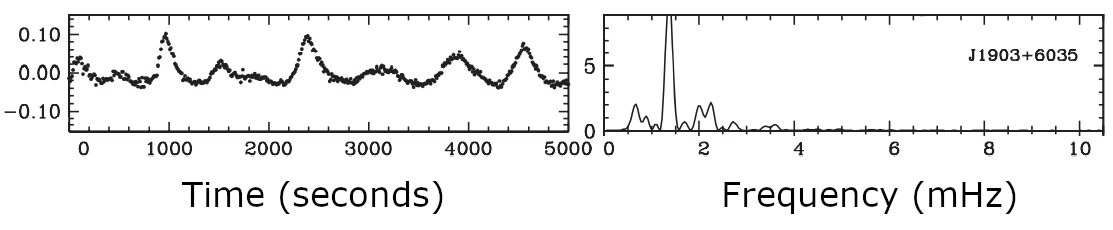
\includegraphics[width=.9\linewidth]{./img/vincent_graph.png}
\caption{\label{fig:vincent}Light curve and Lomb-Scargle periodogrm
  for J1903-6035 adapted from \citet{Vincent_2020} with\emph{out}
  permission.}
\end{figure}
\section{Observation}
We observed J1903+6035 with coordinates RA 19:03:19.56, DEC
+60:35:52.65 and B-band magnitude of 15.5 on a clear moonless night of
May 12, 2021 using the 0.5-m ARCSAT telescope at the Apache Point
Observatory (APO) between 07:09:07 and 11:15:46 UTC. In the airmass
plot shown in Figure \ref{fig:am} the beginning of observation
corresponds to 9 minutes past midnight. According to the
specification, the camera's 16 bit CCD had the gain of 1.25
$e^-/\mathrm{ADU}$ and the read noise of 11.8 $e^-$. The total of 124
raw images with a \SI{100}{\second} exposure were taken through the
\texttt{sdss\_g} filter; however the last 31 images affected by the
approaching twilight had been discarded due to poor quality. Thus the
raw data set consisted of 93 frames covering the interval between
07:09:07 and 10:17:55 UTC, which amounts to the total time span of
\SI{11328}{\second}. While this is at least twice as long as the
observation conducted in \citet{Vincent_2020}, our time resolution is
10 times lower. Most relevant parameters of our observation are
summarized in Table \ref{tab:obs}
\begin{figure}[htbp]
\centering
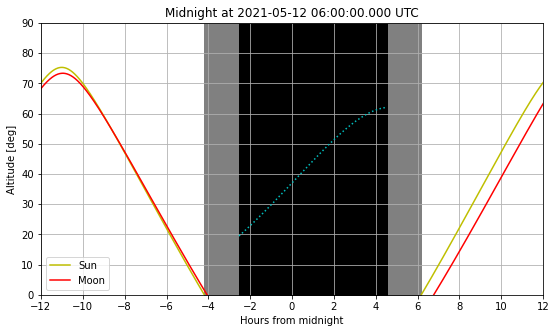
\includegraphics[width=.9\linewidth]{./img/airmass.png}
\caption{\label{fig:am} Airmass plot for J1903+6035 on the night of
  May 12, 2021.}
\end{figure}

\begin{table}
  \centering
  \caption{\label{tab:obs}Observation summary.}
  \begin{tabular}{lr}
    \hline
    Object & J1903+6035 \\
    Coordinates & 19:03:19.56, +60:35:52.65 \\
    Magnitude & 15.5 (B-band) \\
    Date & May 12, 2021 \\
    Start & 07:09:07 UTC (midnight + 00:09:07) \\
    End & 10:17:55 UTC (midnight + 00:17:55) \\
    Exposure & $\SI{100}{\second}$ \\
    CCD & 1024 x 1024 px, 16 bit \\
    Gain & 1.25 $e^-/\mathrm{ADU}$ \\
    Read noise & 11.8 $e^-$ \\
    \hline
  \end{tabular}
\end{table}


Throughout the night, we monitored the quality of the images taken and
at one point needed to intervene and adjust the focus. We decided to
try $\SI{100}{\second}$ exposures even thought we were aware that the
maximum pixel counts corresponding to J1903+6035 never exceeded 3000
ADU. We hoped for another chance at observing and planned on using
slightly longer exposures, but unfortunately the second round of
observation was cancelled due to poor weather conditions.

\section{Data reduction and analysis}
\label{sec:ana}
In addition to the main data set, we also collected bias and flat
field frames; the latter were taking with the same \texttt{sdss\_g}
filter in place. We generated master bias and flat field frames with
the help of the \texttt{ccdproc} Python module and following its
recommended image reduction process from these raw bias flat flat
field frames. In particular, all images including master bias and flat
field frames had been gain-corrected (or converted from the ADU units
into the units of $e^-$) in order to follow the module-recommended
uncertainty propagation practices. Bias has been subtracted from each
gain-corrected image and after that flat-field correction was
performed. Finally, to further improve the quality of the input
images, we employed a median background estimator provided by the
\texttt{photutils} module with the box size of $70\times 70$ pixels;
the estimated background was then subtracted from all the individual
frames producing visibly more uniform field.

To perform differential photometry, we chose 12 reference stars not
significantly different from J1903+6035 in their apparent magnitude
using one of the images (Figure \ref{fig:field}) as the reference
frame. Due to a significant (sometimes exceeding 50 pixels both
horizontally and vertically) shift in the relative positions of the
stars in different frames taken over the course of observation, we
computed a homography transformation between each of the frames and
the chosen reference frame. This was done using the
\texttt{astroalign} Python module. Generally, results were good to
about 1-2 pixels; for better accuracy the coordinates of each star
were optimized via Powell's algorithm (available via \texttt{scipy})
by fitting a narrow 2D Gaussian near the frame-shift-corrected
location of the star prior to applying aperture or PSF photometry
analysis. A reader familiar with photometric techniques and tools may
rightfully point out that a similar out-of-the-box optimization
capability is available via the \texttt{photutils.centroids} module;
unfortunately we weren't aware of its existence when working on this
piece.

\begin{figure}[htbp]
\centering 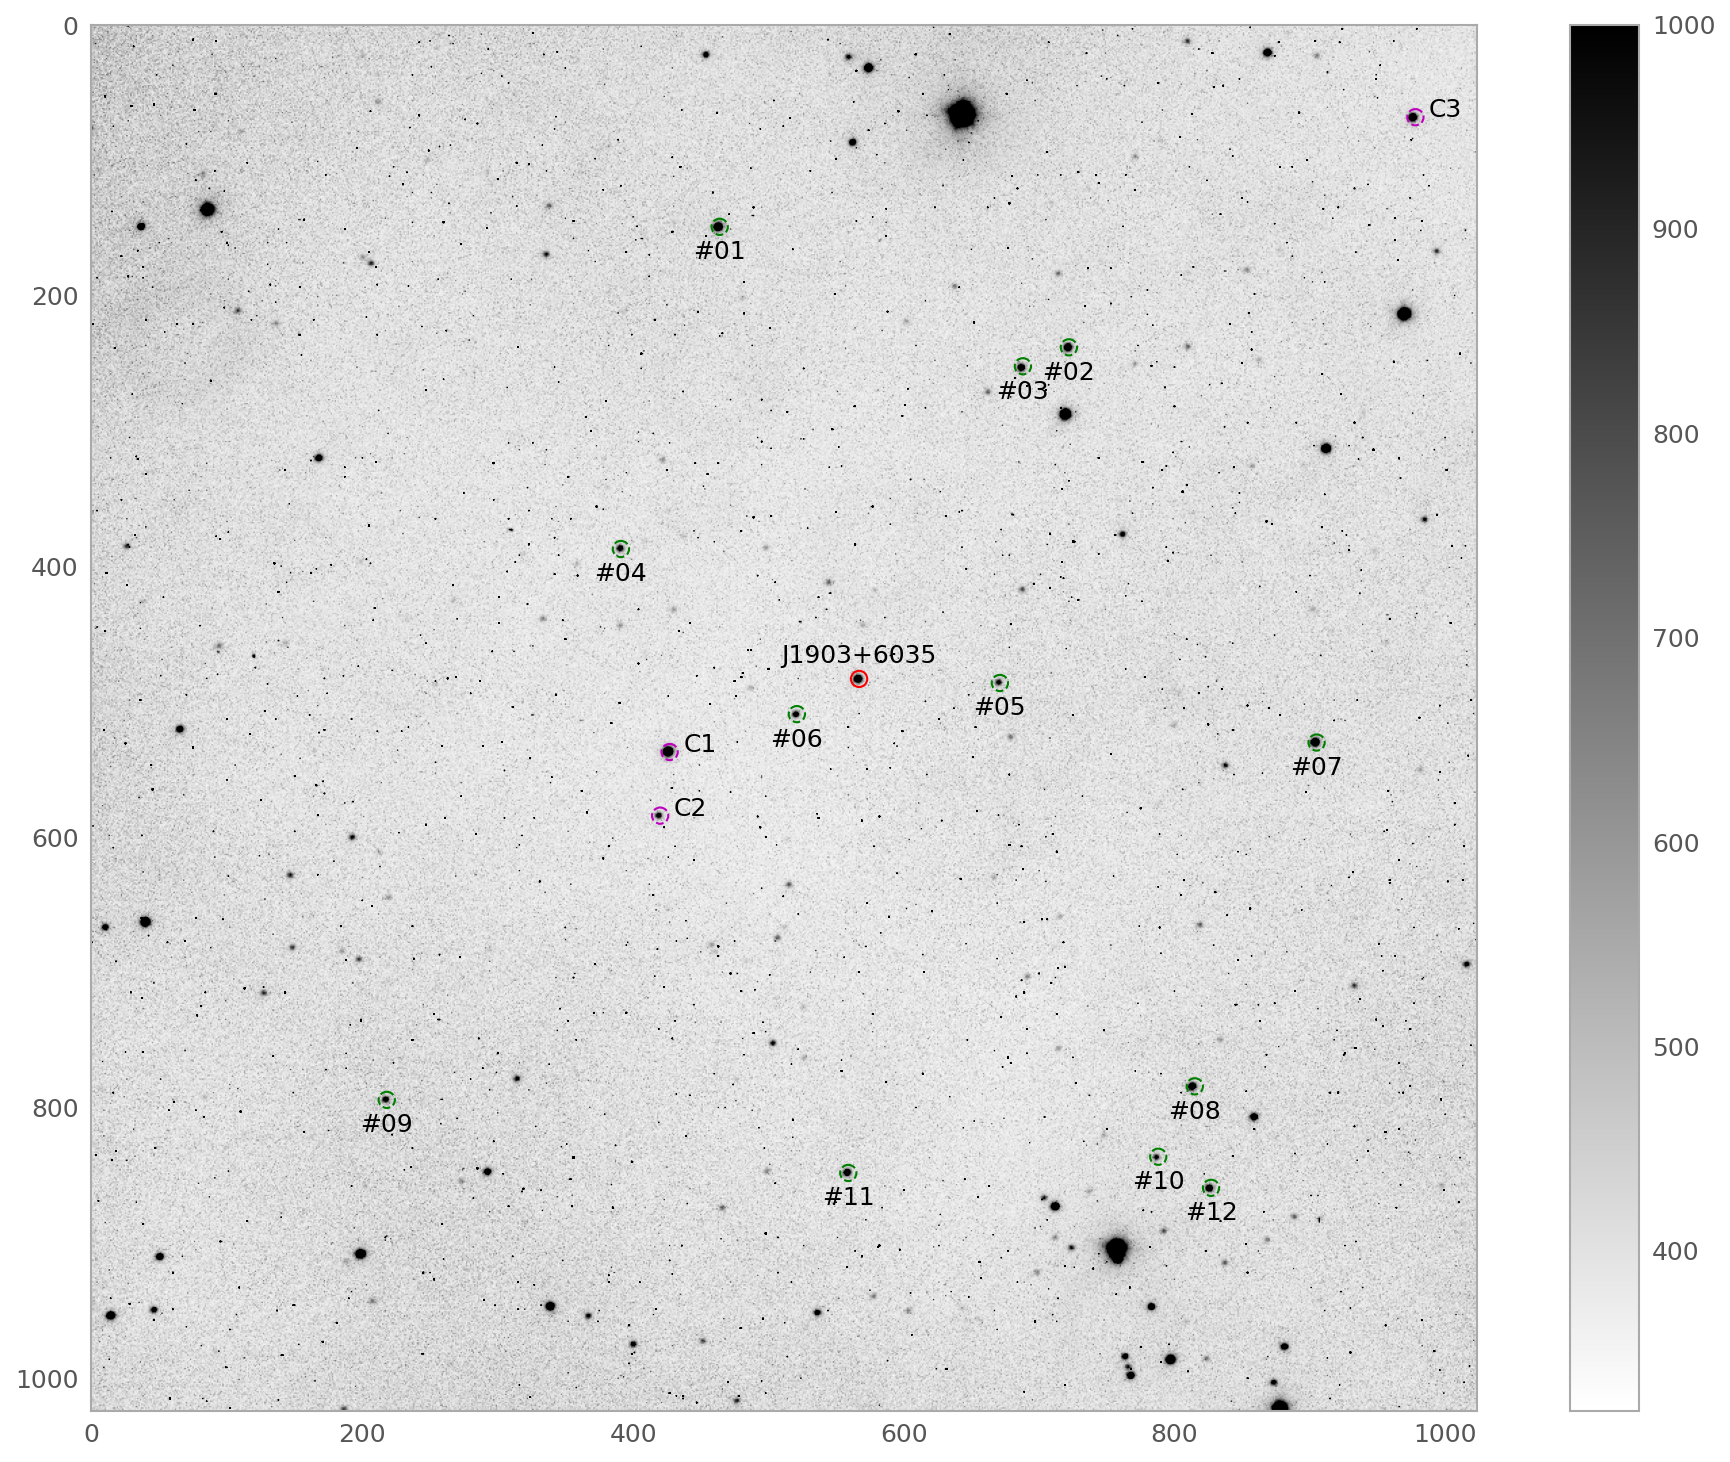
\includegraphics[width=.9\linewidth]{./img/field.png}
\caption{\label{fig:field}Annotated field of view. Stars labeled as
  \#xx are the reference stars, whereas those labeled as Cx are
  control stars. Both reference and control stars, to the best of our
  knowledge, haven't been identified as variable by any astronomical
  survey.}
\end{figure}

The differential photometry procedure was performed as follows: the
flux (in the units of $e^-$ due to the gain correction mentioned
earlier) was computed via aperture (and also PSF) photometry method
for the main and reference stars in each of the frames; then the
relative flux of the main star was determined as the ratio of its flux
and the average flux of all the reference stars. The resultant light
curve is shown in Figure \ref{fig:lc}.

\begin{figure}[htbp]
\centering
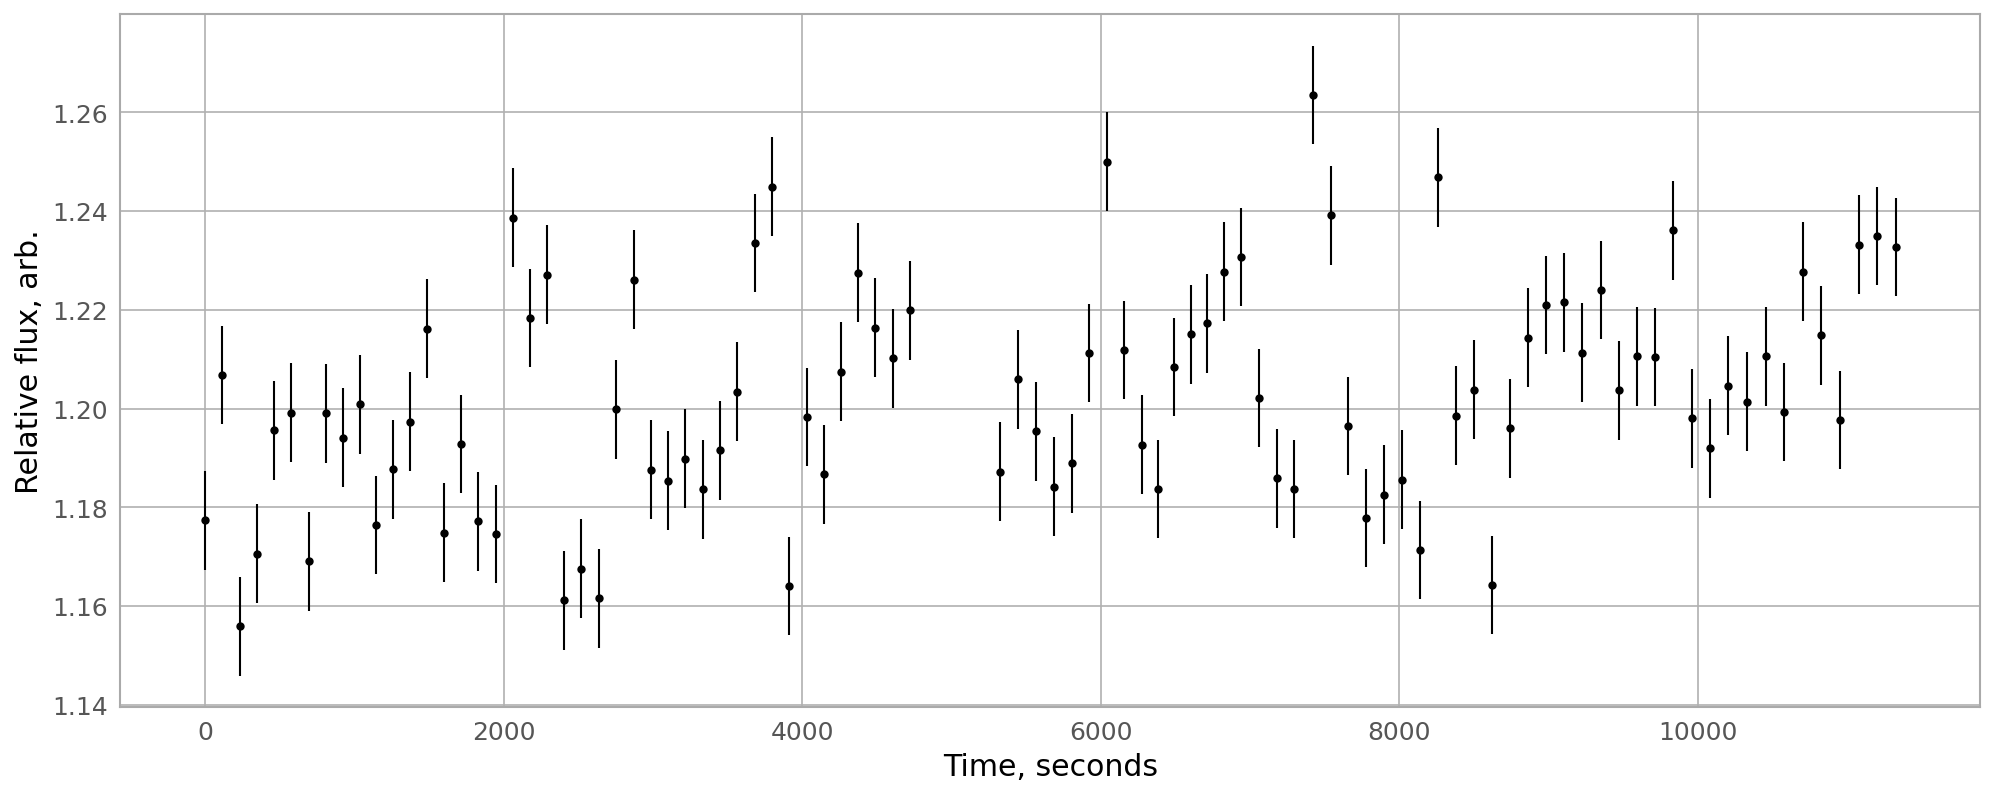
\includegraphics[width=.9\linewidth]{./img/lightcurve.png}
\caption{\label{fig:lc}Light curve of J1903+6035. Variation of the
  relative flux of J1903+6035 with respect to its mean value. Values
  of several consecutive data points missing due to a technical issue
  during data acquisition were imputed in order to apply FFT spectral
  analysis.}
\end{figure}

As seen from the light curve in Figure \ref{fig:lc}, typical time
intervals between successive measurements were approximately uniform
(with $\Delta t=\SI{118\pm4}{\second}$), so it isn't unreasonable to
expect that the dominant modes' frequencies will be prominent in the
power spectrum, which can be produced via Fast Fourier Transform
(FFT). The result of the FFT spectral analysis is shown in Figure
\ref{fig:ps}. Note that due to a technical issue, there was a
discontinuity in the light curve data with multiple missing data
points (see Figure \ref{fig:lc}, near
$t\approx\SI{5000}{\second}$). Since FFT is unable to handle
discontinuities in the data and expects evenly spaced data points, we
filled the gap with imputed values spaced similarly to the rest of the
data set and set equal to the data set average, which in this case,
after the mean value was subtracted from the data to suppress the zero
frequency component in the power spectrum, was simply zero. Given our
sampling frequency of approximately \SI{8}{\milli\hertz}, the Nyquist
frequency is about \SI{4}{\milli\hertz}. This means our analysis will
not be able to detect frequencies faster than that (which means we are
unable to detect periods shorter than \SI{250}{\second} due to
aliasing).

\begin{figure}[htbp]
\centering
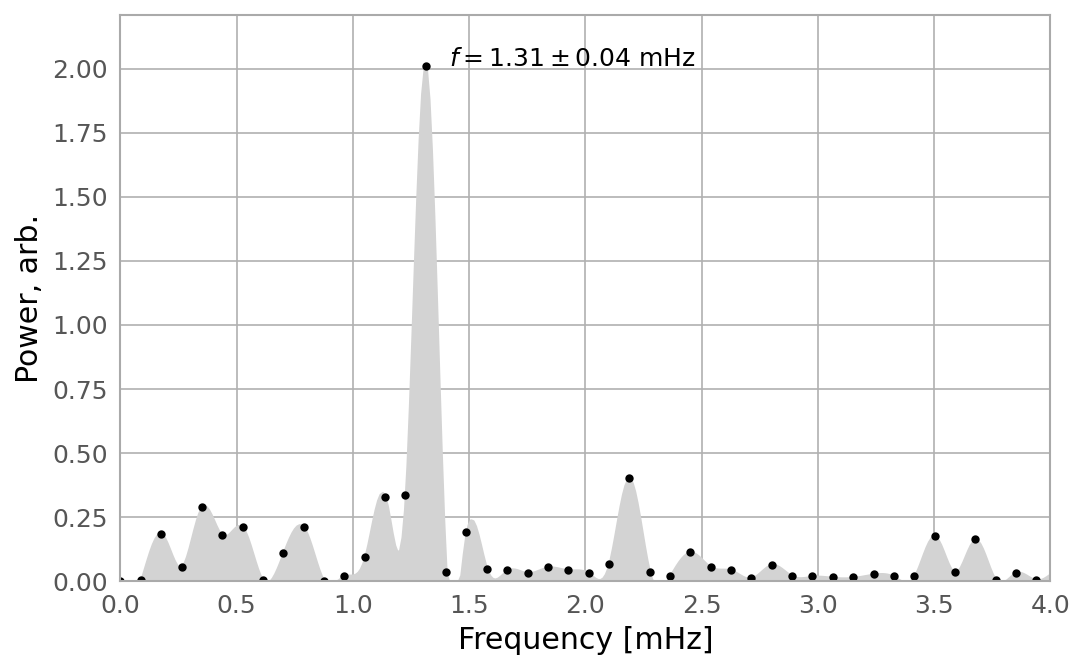
\includegraphics[width=.9\linewidth]{./img/power.png}
\caption{\label{fig:ps}Power spectrum of the relative magnitude of J1903+6035.}
\end{figure}

From the power spectrum in Figure \ref{fig:ps}, it is unambiguously
clear that the sharp peak near $f=\SI{1.31\pm0.04}{\milli\hertz}$
constitutes the dominant mode, which corresponds to the period
$P=\SI{763\pm 23}{\second}$. Since the peak is so sharp, it was
reasonable to estimate uncertainty in frequency by taking one half of
the FFT frequency step (i.e., $\Delta
f\approx\SI{0.08}{\milli\hertz}$) and estimating the uncertainty in
the period based on the uncertainty in the frequency using the simple
first-order formula
\[
  \delta P\approx \frac{1}{f^2}\delta f.
\]
It must be noted that without imputing the missing data points the
peak would appear much less prominent and sharp, which isn't
surprising given that FFT is very sensitive to shifts and
irregularities in the intervals between successive data
points. Frequencies slower than \SI{0.5}{\milli\hertz} would
correspond to periods longer than \SI{2000}{\second}, which are much
longer than what we would expect and also aren't reliable since our
data would cover fewer than 5 full periods. Spectral analysis via FFT
is a quick and easy tool to apply, but it must be noted that due to
the small but non-negligible variability in the intervals between
successive data points, the result (which assumes a series of values
evenly spaced in time) should be interpreted with caution. Generalized
Lomb-Scargle periodogram would be a more appropriate technique for
deriving the period from this data because unlike FFT is doesn't
expect evenly spaced data, which also means we do not need to impute
missing data points. Moreover, the Lomb-Scargle algorithm available
via the \texttt{astroML} package provides means of estimating
statistical significance of the result through the bootstrap
method. In regard to periodograms, this method is based on repeated
resamping while keeping the time coordinates the same. The data points
are taken randomly with replacement from the observed values, and then
the maximum of the resulting periodogram is computed. Bootstrap gives
the most robust estimate of the false alarm probabilities because it
makes very few assumptions about the form of the distribution
\citep{VanderPlas_2018}.

A generalized Lomb-Scargle periodogram obtained from the light curve
in Figure \ref{fig:lc} is shown in Figure \ref{fig:lsp}. Note that it
echoes the power spectrum in Figure \ref{fig:ps} discussed earlier
confirming the presense of a dominant mode with period of $\SI{765\pm
  29}{\second}$ with very low false alarm probabilty. The uncertainty
was determined, following the discussion in \citet{VanderPlas_2018},
by taking the half-width at half-maximum of the dominant peak in the
periodogram. This is in great agreement with the result obtained via
FFT spectral analysis, which means we can rely on the significantly
more computationally efficient FFT in the following complementary
analysis.

\begin{figure}[htbp]
\centering
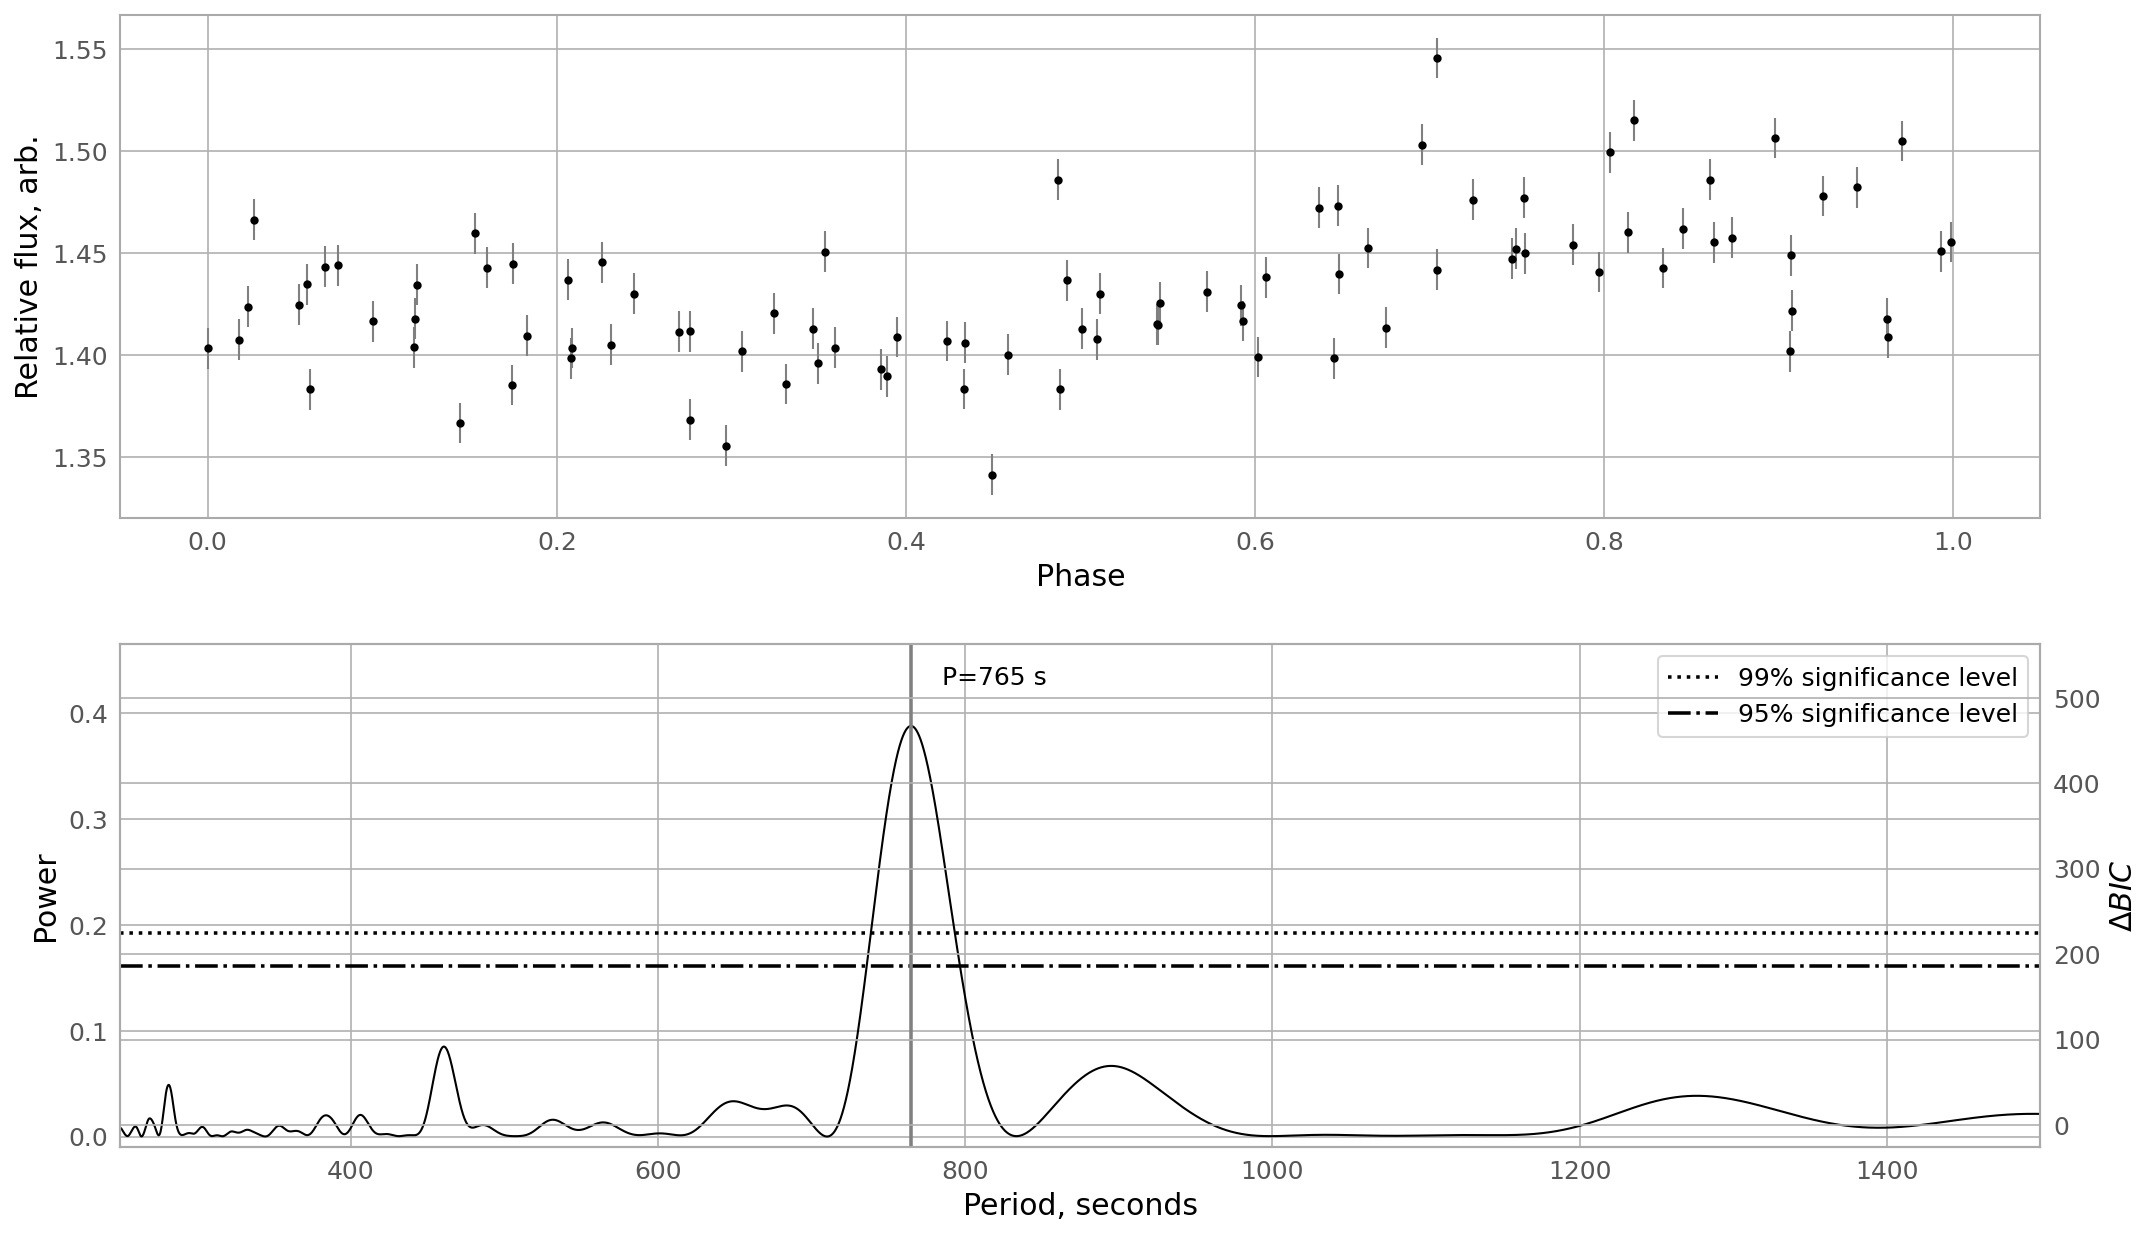
\includegraphics[width=.9\linewidth]{./img/ls_periodogram.png}
\caption{\label{fig:lsp}Lomb-Scargle periodogram of the relative
  magnitude of J1903+6035.}
\end{figure}

To further validate the statistical significance of this result and
confirm that it didn't arise from an error in the analysis, variation
of the flux of the reference stars, or some unknown digital artifact,
we perform the same data reduction procedure again, but having
J1903+6035 replaced with different stars which haven't been identified
as variable by any astronomical survey. These "control group" stars
are marked as C1--C9 in Figure \ref{fig:field}. The power spectra
corresponding to these stars produced in the same way as that for
J1903+6035 are shown in Figure \ref{fig:control}. (It is worth
mentioning that the light curves of the control stars where produced
together with that for the main star. Computing a homography
transformation for each frame and subsequently fine-tuning the
coordinates of all the stars is a rather computationally expensive
task. Repeating these steps for each control star would require
significant processing time and therefore should be avoided. Moreover,
it was possible to drastically improve the efficiently of the
photometry analysis by relying on Python's \texttt{multiprocessing}
module to enable parallel processing of individual frames; generally,
this allows reducing the overall processing time by a factor equal to
the number of available CPU cores.)

It is evident that all 9 control star power spectra shown in Figure
\ref{fig:control} are devoid of prominent features with frequencies
higher than $f\approx\SI{0.5}{\mHz}$. This indicates that no
significant variation with a period shorter than about
$\SI{2000}{\second}$ has been detected for any of the control
stars. We also performed a confirmatory Lomb-Scargle periodogram
analysis on each of the control stars. It did not report any even
slightly statistically significant variation having a period
comparable with $\SI{765\pm 29}{\second}$ (in fact, no statistically
significant variation was reported at all for all the control stars);
since the periodograms didn't reveal any notable features, we chose
not to present them here.

\begin{figure}[htbp]
\centering
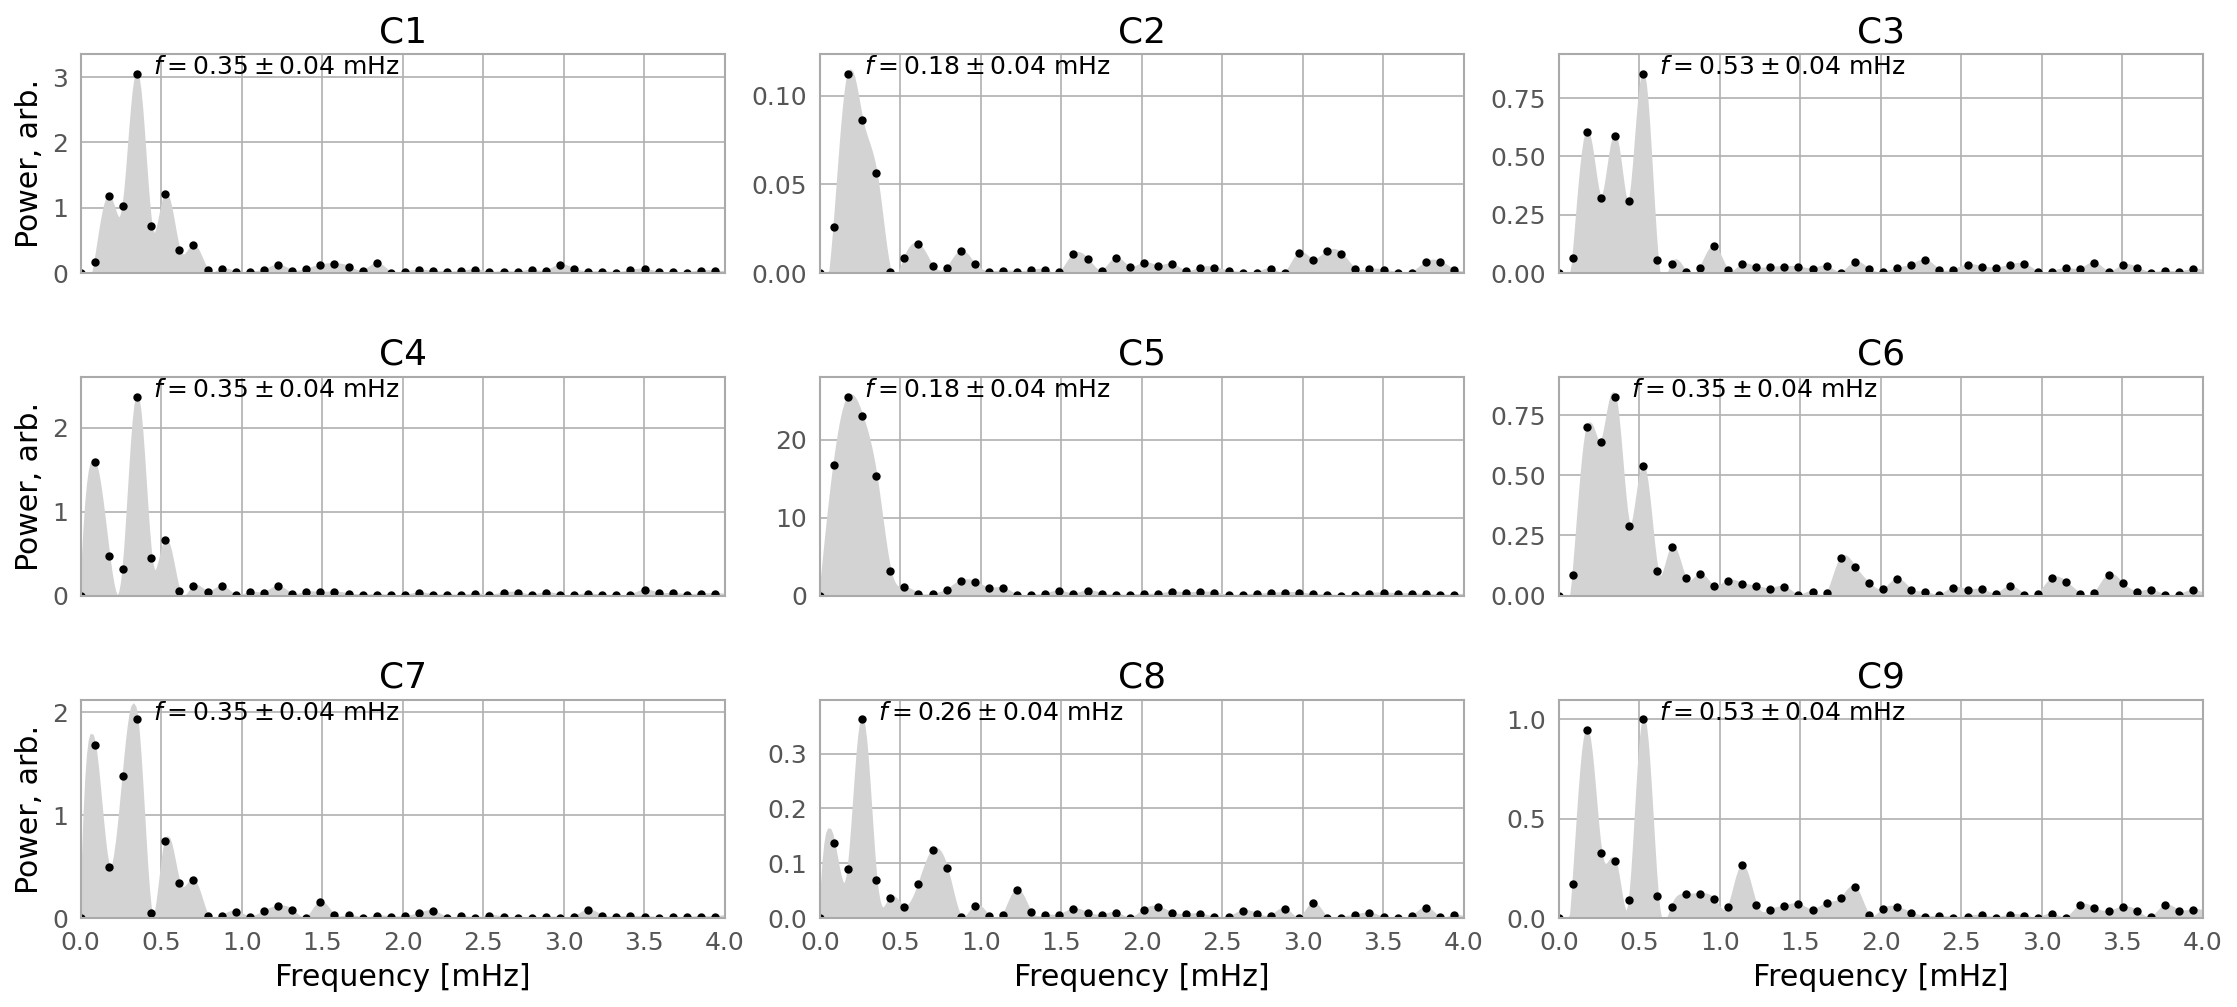
\includegraphics[width=.9\linewidth]{./img/control.png}
\caption{\label{fig:control}Power spectra of the control stars.}
\end{figure}

It didn't escape our notice that the differential light curves for all
the control stars appeared to be strongly correlated. This fact was
evident from simply inspecting the light curves and also from the
apparent similarity of the power spectra shown in Figure
\ref{fig:control}. In fact, the average light curve of all the control
stars and the corresponding power spectrum shown in Figure
\ref{fig:avg} reveal the shape of a low frequency signal whose most
salient time-domain features can now be easily identified even in the
light curve of J1903+6035 shown in Figure \ref{fig:lc}. While we don't
know what exactly is the source of this pervasive signal, we suspect
it may be related to the variation in the telescope's point spread
function (PSF) over time and also the rotation of the worm gear of the
telescope drive. While taking the data, we noticed obvious signs of
astigmatism manifest in slightly asymmetrical shape of the stars
(Figure \ref{fig:psf}). We also noticed a dynamic shift in the axis of
astigmatism, or time-varying discrepancies in the focus along the
horizontal and vertical axes. Due to this, the shapes of the stars
appeared elliptical with time-varying aspect ratio and incline of the
major axis. At one point, hoping to mitigate this effect and improve
the quality of the images, we decided to readjust the focus. This
manual intervention was the reason several out-of-focus frames around
$t=\SI{5000}{\second}$ in into the observation had to be discarded. We
suspect this parasitic signal arose from the variation in the focus
and astigmatism (and therefore PSF), possibly in combination with the
effects from operating close to the noise floor of the CCD; even with
the exposure as long \SI{100}{\second} the peak counts for J1903+6035,
an average star among other stars used either as a reference or
control, were always slightly below 3000.

\begin{figure}[htbp]
\centering
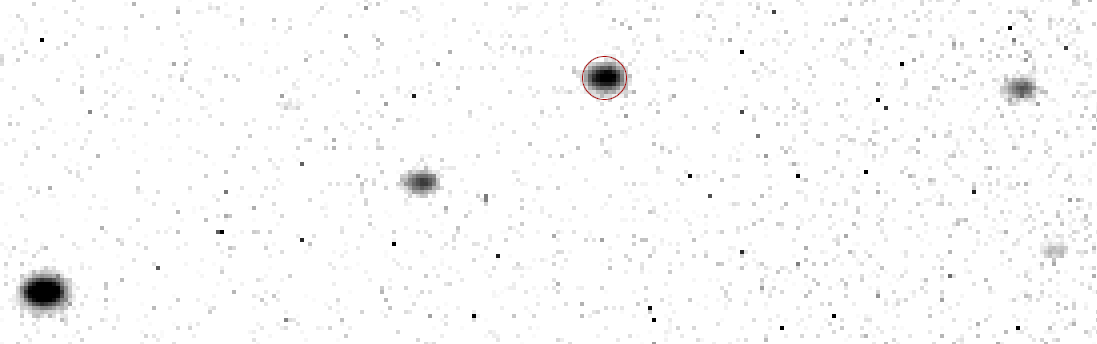
\includegraphics[width=.4\linewidth]{./img/psf.png}
\caption{\label{fig:psf}Elliptical PSF due to optical astigmatism. The
  red circle shows the approximate size of an aperture with 5 pixel
  radius on top of J1903+6035. This aperture is appropriate for the
  main star, but may be smaller than ideal for some of the bright
  reference stars, which together with time variation of the shape of
  the PSF could be the culprit of the parasitic signal.}
\end{figure}

\begin{figure}[htbp]
\centering
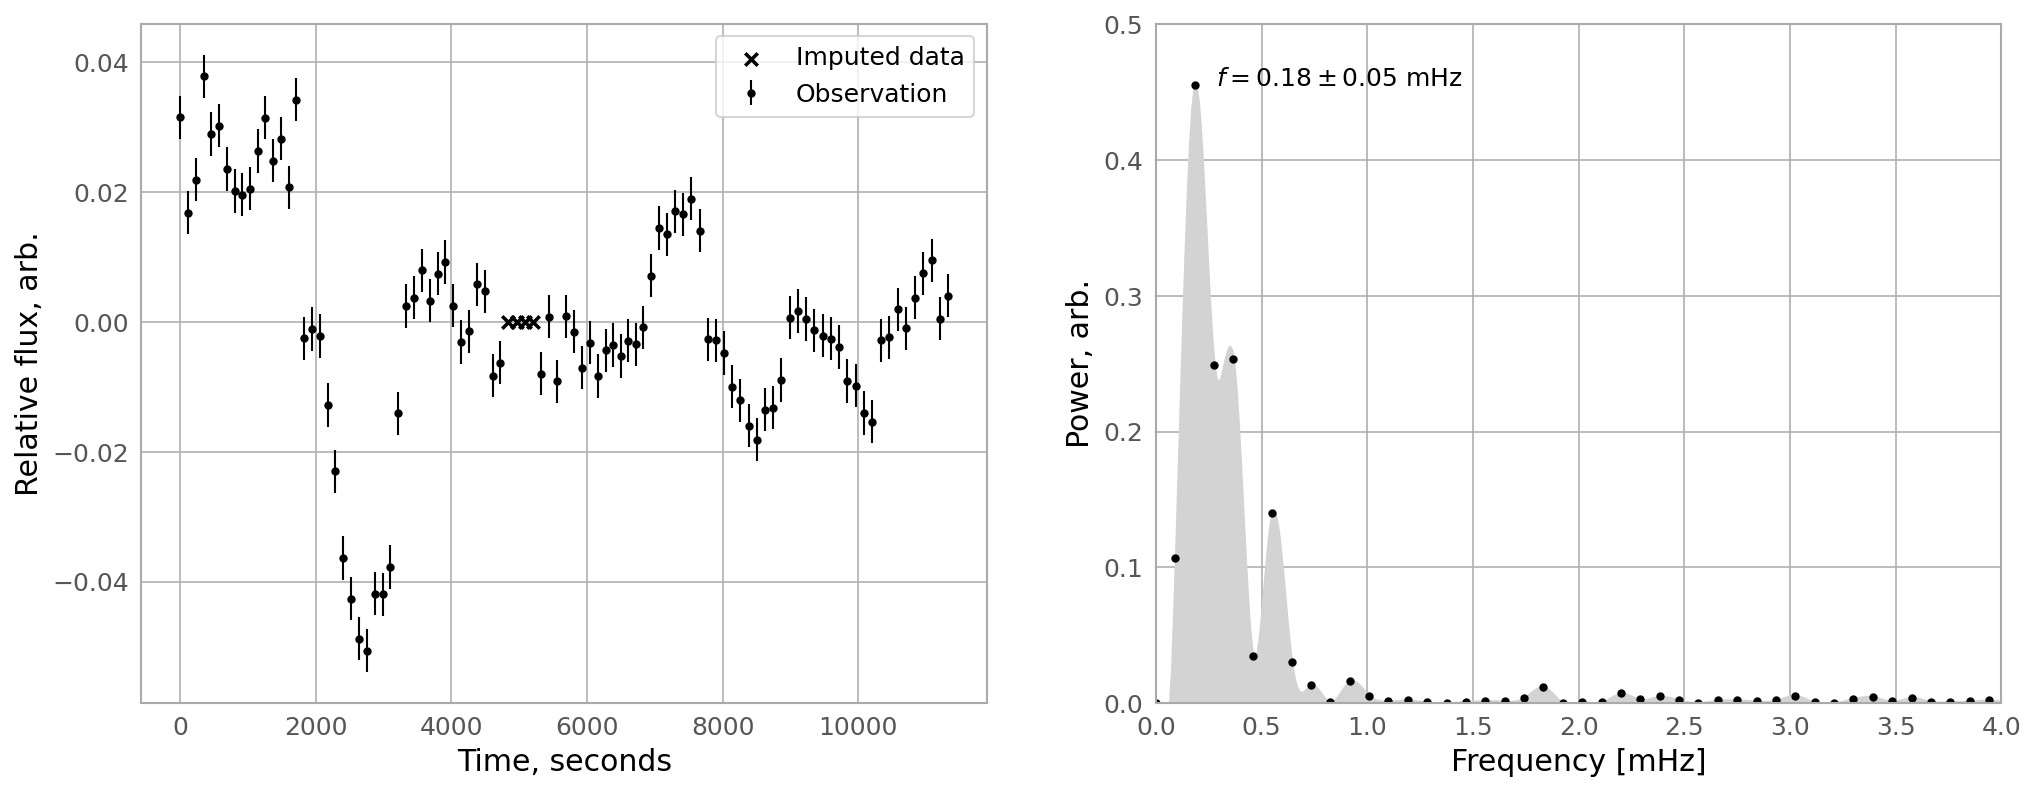
\includegraphics[width=.9\linewidth]{./img/average.png}
\caption{\label{fig:avg}Average lightcurve of the control stars
  C1--C9. This shows the overall shape of a parasitic signal which may
  be attributed to poor calibration of the optical system.}
\end{figure}

Despite the presence of the parasitic signal, the fact that no control
star exhibited any even slightly prominent variation with a frequency
close to the one determined for J1903+6035 earlier suggests that
detected variation was not due to any artificial signal and is,
indeed, more likely than not due to the actual variation in brightness
caused by \emph{g}-mode oscillations. It is, perhaps, a lucky
coincidence that the frequencies of the target and parasitic signals
were different enough to preclude any significant interference.

In view of the discussion about the technical issues encountered
during data acquisition, it should now be clear why aperture
photometry was chosen in favor of PSF photometry. The PSF suitable for
our data set would have to be a complex time-dependent function in
order to adequately compensate for poor focus, astigmatism and
possibile non-linear CCD response effects. Aperture photometry with a
relatively large radius of 5 pixels, while more prone to be affected
by noise, was good at consistently estimating the relative flux across
this generally inhomogeneous data set. It is, however, worth
mentioning that we did attempt photometry using a circular Gaussian
PSF. The final results of such analysis were essentially identical to
those produced via aperture photometry, althought the peaks in the
power spectra of J1903+6035 appeared notably less promiment.
\section{Discussion}
According to independent spectroscopic measurements
\citep{Limoges_2015}, J1903-6035 has the following effective
temperature and mass: $T_{\mathrm{eff}} = \SI{10858\pm 63}{\kelvin}$,
$M=0.624\pm 0.006 M_\odot$. This puts it at the about the center of ZZ
Ceti instability strip, slightly toward its red edge. It is known that
the amplitude of the dominant mode diminishes as the star approaches
closer to the red edge of the instability strip; however, this effect
doesn't set in until the period exceeds about $\SI{800}{\second}$
\citep{Vincent_2020}. This is consistent with the fact that the
amplitude of variation of J1903-6035 as estimated in
\citet{Vincent_2020} was as large as 10\% of the mean brightness of
the star. Unfortunately, due to extremely poor signal-to-noise ratio
and the presence of a parasitic signal, we were not able to reliably
estimate the amplitude of the dominant mode.


The average pulsation period of J1903+6035 given by
\citet{Vincent_2020} is $\SI{726}{\second}$, whereas our value is
$\SI{765\pm29}{\second}$. While our period is somewhat longer, the
difference is hardly statistically significant. In fact, it is easy to
see that the last 4 somewhat ``regular'' peaks in the light curve
shown in Figure \ref{fig:vincent} span the interval of about
$\SI{2400}{\second}$. This interval constitutes 3 full periods, which
means the average period on this segment should be close to
$\SI{800}{\second}$.

As discussed in \citet{Kepler_1983}, is it very difficult to
accurately determine the modes of a ZZ Ceti star, which often tend to
be very close to each other (for reasons which will be discussed
shortly). This means that as the relative phase between the two
closely spaced modes slowly accumulates over time, observations can
vary quite substantially from one night to another. This is
complicated by the fact that the amplitude and phase of the
\emph{g}-modes generally tends to be unstable \citep{Bergeron_1990}
partly because of the slow rotation of the star, but also as a result
of complex non-linear interaction between competing driving
mechanisms. Therefore, truly resolving the modes would require
sampling frequencies and optical sensitivities far beyond our
reach. It is, however, quite remarkable that our analysis, despite the
challenges encountered during data acquisition was able to isolate an
extremely weak signal from noise and undesirable artifacts.

An order-of-magnitude estimate of the period of pulsation of a white
dwarf star based on the the classical theory of pulsating stars
(applicable, for instance, to Cepheid variables) is based upon
relating the time for sound to travel across the star to its pulsation
period. The general form of this relationship, ignoring constant
factors which are close to 1, is given by

\[
\mathcal{P} \sim (G\bar\rho)^{-\frac{1}{2}},
\]
where $\bar\rho$ is the average density of the star
\citep{Winget_2008, Catelan_2015}. Considering that the average
densities of white dwarfs are in the range between $10^7$
$\SI{}{\kilogram\per\meter^3}$ and $10^{10}$
$\SI{}{\kilogram\per\meter^3}$ (or typically about $10^9$
$\SI{}{\kilogram\per\meter^3}$), this suggests that the periods of
pulsation should be no longer than $\SI{40}{\second}$ (or about
$\SI{4}{\second}$ for most typical stars). Clearly, this
underestimates the observed periods by about two orders of
magnitude. This discrepancy has puzzled the astronomers for a long
time, until it was suggested that ZZ Ceti stars (as well as other
pulsating white dwarfs) exhibit non-radial gravity- or \emph{g}-mode
pulsations which are much slower than the radial pressure
(\emph{p}-mode) oscillations.

While giving a comprehensive theoretical treatment of pulsating white
dwarfs is far beyond the scope of this work, we would like to provide
at least minimal intuition into the physical nature of non-radial
\emph{g}-mode pulsations. The general idea is that such pulsation (in
contrast with purely radial ones) distort the spherical symmetry of
the star. This means that while some areas of the star's surface
expand, others contract. This is similar to waves on the surface of a
pond: when fluid is displaced from its equilibrium position (for
instance, by wind), gravity tries to return it back to equilibrium,
which results in oscillations. The general consensus in the literature
is that the \emph{g}-mode pulsations on the surface of DAV (ZZ Ceti)
stars are driven by partial ionization of hydrogen (which is the most
abundant element in DA type stars) and, as was suggested in
\citet{Dziem_1981}, by $\delta$ mechanism also known as
\emph{convective driving}. The observed instabilities in the
amplitudes and phases of the \emph{g}-modes are commonly attributed to
the non-linear interaction between ionization and convection
mechanisms and couplings between different pulsation modes
\citep{Bognar_2009}.

As for any wave phenomenon occurring over the surface of a spherical
body, it is natural to model \emph{g}-mode pulsations using spherical
harmonics $Y_{lm}$. Suppose the frequency of pulsation of a
non-rotating ZZ Ceti star corresponding to some $l>0$ is
$\sigma_l$. Then clearly the observed frequencies corresponding to all
possible values of $m\in-l..l$ would be identical. This degeneracy is
lifted in stars that rotate, which provides a simple means of
estimating the rotation angular frequency $\Omega$ of the star using
the following relation valid to the first order in $\Omega$
\citep{Fu_2013}:
\[
\sigma_{lm} = \sigma_l + m\left(1 + \frac{1}{l(l+1)}\right)\Omega.
\]
Most ZZ Ceti stars are relatively slow rotators with periods on the
order of one to a few days, as was confirmed via many independent
measurements. It is also possible to infer, using geometric arguments,
the incline of the rotation axis of the star relative to the line of
sight by considering the relative amplitudes of the modes
corresponding to different values of $m$; however, this technique must
be used with caution since it assumes that the symmetry axis or
pulsations coincides with the rotation axis of the star itself
\citep{Fu_2013}.

Apart from determining the rotation periods of stars, there are many
other reasons why accurate resolution of the pulsation modes of ZZ
Ceti stars is important. For instance, cooling timescale of white
dwarfs are directly proportional the timescale of their period
changes. This can be instrumental in estimating the birth rates of
white dwarfs taking into account their abundance, which in turn gives
an estimate of the age of the galactic disk. In addition to that, the
cooling timescale is linked to the core composition of white dwarfs
via the equation of state \citep{Koester_1990}, which can provide a
window into the structure and evolution of such stars
\citep{Kepler_1989}.

This brief survey of the \emph{ZZ Ceti} research was provided to
emphasize the importance of acquiring high-quality time-lapse
photometric data sets and making them available to astronomers, in
particular, astroseismologists studying pulsating white dwarfs. The
merit of conducting observations and data analyses similar to the one
showcased in this work is not in the quality of the raw data and the
accuracy of the results. Small telescopes like ARCSAT clearly wouldn't
be able to produce data with sufficient time resolution and adequate
SNR. We argue that the merit is in the relatively cheap identification
of potentially interesting \emph{ZZ Ceti} targets for more
comprehensive observation using larger professional
telescopes. Currently, to the best of our knowledge, no comprehensive
catalogue of DAV stars and their parameters exists, which makes it
rather difficult for astroseismologists to validate their models and
advance the theoretical understanding of these still in many ways
mysterious objects.

With the goal of presenting this work as a field guide to those
amateur astronomers who are interested in identifying new \emph{ZZ
Ceti} stars using small telescopes similar to ARCSAT, we now focus our
discussion on the technical details and potential problems one may
encounter when conducting similar surveys. Unfortunately, it rained on
one of the two nights during which we had been scheduled to observe
and for that reason we were unable to acquire another data set. Had we
been given the opportunity to observe J1903-6035 again, we would
certainly address the astigmatism and focus issue which almost
thwarted all our efforts in confirming the star's variability. In
addition to that, since we suspected non-linear CCD response to be
another possible contributor to the parasitic signal, it may be
worthwhile to increase the exposure time such that the counts are
higher above the noise floor. This would naturally compromise the
already low time resolution, but if it helps eliminating the parasitic
signal, it may still be produce overall better data without unwanted
artefacts. Counts could also be increased by not using any filter; in
fact, that is exactly what \citep{Vincent_2020} did when conducting
their survey. Apart from lowering the counts, our \texttt{sdss\_g}
filter introduced exposure irregularities, which were only partially
corrected using flat fields and background estimation. It is not
entirely impossible the the parasitic signal arose from these exposure
irregularities combined with shifts of the view field throughout the
observation. (This hypothesis can be relatively easily verified, even
without additional observation, by looking for correlation between
frame shift and the parasitic signal; unfortunately due to time
constraints we cannot pursue such analysis at this time.)

The data reduction and analysis methods described in Section
\ref{sec:ana} are fairly standard. However, our attempts to identify
cosmic rays via the L.A. Cosmic technique (implemented in
\texttt{ccdproc}) didn't succeed and were abandoned; in future
iterations of this analysis, we would like to revisit cosmic ray
identification and removal. So far we discussed multiple hypotheses as
to the origin of the parasitic signal, each having to do with the
process of observation. We can't, however, completely rule out the
possibility that it was introduced at some point during the data
reduction or was somehow inherent in the signal associated with one or
more reference stars. Therefore, we plan to take a closer look at our
random selection of the reference stars and study how it affects the
shape and strength of the parasitic signal. A slim chance still
remains that one of our reference stars was, in fact, variable and the
parasitic signal was real. Our quick experimentation with the choices
of reference stars didn't seem to support this idea; it showed that
the parasitic signal was there regardless of what stars we used for
reference. We did, however, observe a correlation between the strength
of the parasitic signal and the spread in the apparent magnitudes of
the reference stars, which was in line with our previous attribution
of the parasitic signal to time-varying PSF and non-linear CCD
response close to the noise floor.

Finally, we would like to highlight a few techniques which resulted in
a substantial increase in the statistical significance of the end
result. When conducting similar analyses in the future, we will likely
continue relying upon these tool, only adding incremental
improvements. The computation of a homography transformation to align
the stars and subsequent fine-tuning of the coordinates proved to be
much more computationally efficient and accurate than the source
detection facilities offered by \texttt{photutils}. As was already
discussed, aperture photometry (using optimized source coordinates)
produced good results. We tried different aperture radii between 4 and
8 pixels and were able to obtain qualitatively and quantitatively
identical results to the ones reported. The best results were achieved
with the radius of 5 pixels; the prominence of the dominant peak in
the power spectra diminished whenever we deviated from this
``optimal'' value. If the images in the data set a not severely
impacted by astigmatism or other optical abberrations, radii as small
as 3 pixels should be ideal. Obtaining power spectra via FFT is very
easy (when using \texttt{scipy}) and computationally efficient;
however it is extremely important that the data points be equally
spaced. Our imputing several missing values drastically improved the
resolution of the power spectra. (Of course, ideally, there should not
any gaps in the time series data.) To our surprise, using the
background estimator helped produce much cleaner power spectra. In the
future we would like to gain better understanding of how to estimate
and subtract the background optimally --- i.e., what values of box and
filter size as well as what clipping technique produce best results.

\section{Summary and conclusions}
In this paper we confirmed that the J1903-6035 star is variable and
has a dominant mode with period of $\SI{765\pm 29}{\second}$ which
agrees, within uncertainty, with the initial estimate in
\citet{Vincent_2020}. We provided a detailed discussion of a data
reduction technique, which allows identifying candidate \emph{ZZ Ceti}
stars for further detailed study even when the observation is
performed with small-aperture telescopes. Even with access to a large
telescope, resolving different modes of pulsation would require many
hours of observation on multiple nights as discussed in
\citet{Winget_2008}, \citet{Kepler_1989} and
\citet{Bergeron_1990}. This is expensive, so there's clear benefit in
performing the initial identification of interesting targets using
small telescopes not involved in ``serious'' astronomical
research. Several technical difficulties which significantly
compromised the quality of our raw data are identified and suggestions
are made about avoiding them in the future (see Section
\ref{sec:ana}).

We believe that acquiring high-resolution data sets and conducting
analyses aimed at accurately resolving as many \emph{g}-mode
oscillation frequencies as possible is essential to advance our
currently incomplete theoretical understanding of the important phase
in the evolution of white dwarfs --- their passage through the
\emph{ZZ Ceti} instability strip. Moreover, we briefly discuss several
indirect observations, which become possible if accurate values of
pulsation mode frequencies are known. We provide brief insights into a
few examples of such observations: the inference of the angular
frequency of the star from the splitting of the degree $l$ modes;
estimate of the axial tilt of the star based on the relative amplitude
of different modes; determination of cooling time scales of the white
dwarfs based on the variations in the mode frequencies over time,
which in turn serves as a proxy when estimating the age of the
galactic disk.

All calculations in this paper were performed using Python and
open-source packages. The two major steps of the data analysis are
initial photometry and time series reduction. The output of the former
is the light curve for the main and control stars produced via
differential photometry, whereas the output of the latter is the final
result deduced from both FFT and Lomb-Scargle periodogram spectra with
the control stars used to refute the null hypothesis. Both parts or
the analysis are implemented as configurable software, which can be
reused when conducting a similar survey. All source code used to
produce the results and figures presented in this paper is freely
available on GitHub\footnote{The source code and notebooks are
available at
\url{https://github.com/wdecay/ASTR480/tree/master/project}} in the
form of standalone Python modules and Jupyter notebooks.

We are grateful to Conor Sayres for assisting us with the ARCSAT
telecope, and also to Professor Sarah Tuttle, Tae Yokota and Mira Cho
for helpful feedback on early drafts of this paper.

\bibliography{refs}{}
\bibliographystyle{aasjournal}

\end{document}
